\chapter{Лекция №6 - 25.03.2021. Страхование не-жизни} % (fold)

В случае страхования \textbf{ не-жизни} имеем дело с двумя случайными величинами
\begin{enumerate}
	\item число требований (страховых событий)
	\item размер выплаты по каждому требованию (необязательно полное уничтожение имущества, а значит \red{страховое возмещение } $\leq$ \red{ страховой суммы})
\end{enumerate}

\red{Страховая сумма } - верхний предел ответственности страховой комапании перед страхователем.

\begin{remark}
	Договор страхования заключается не более чем на год
\end{remark}

Пусть
\[ X = x_1 + ...+ x_n - \]
сумма всех выплат по одному страховому полису (застраховав машину на год, мы можем несколько раз за год попасть в аварию).

Тогда $EX$ - \red{ нетто-ставка}, но в non-life insurance за основу берется \red{ риск-ставка}
\[ r = \pi(x) = EX + \rho, \]
где $\rho$ - \red{ рисковая надбавка}.

\textbf{Как искать рисковую надбавку?}

Нельзя дать слишком маленькую (ведёт к разорению страховой компании) или слишком большую (вытеснению с рынка из-за конкуренции) рисковую надбавку.

Имеются следующие правила расчета риск-ставки:
\begin{enumerate}
	\item \textbf{принцип математического ожидания}
	\[\pi(x) = EX + \alpha EX\]
	\item \textbf{принцип стандартного отклонения}
	\[\pi(x) = EX + \beta\sigma,\;\;\;\sigma = \sqrt{DX}\]
	\item \textbf{принцип дисперсии}
	\[\pi(x) = EX + \gamma\sigma^2\]
	\item \textbf{комбинированный способ}
	\[\pi(x) = EX + \beta\sigma + \gamma\sigma^2\]
\end{enumerate}

Эти правила основаны скорее на интуиции и здравом смысле, чем на глубоких теоретических принципах. Их часто называют \red{ прагматические принципы}.

Окончательно с клиента берется \red{коммерческая премия} или \red{брутто-ставка}, которая состоит из \textbf{риск-ставки} и \textbf{нагрузки}.

Нагрузка включает в себя:
\begin{enumerate}
	\item расходы на ведение дел $\sim 15\%$
	\item предупредительные мероприятия $\sim 10\%$
	\item прибыль $\leq 15\%$
\end{enumerate}

В случае имущественного страхования нагрузка равна $\sim 15\% + 10\% + 15\% = 40\%$ от коммерческой премии.

\section{Модели учета риска} % (fold)


% section модели_учета_риска (end)
Полис может составляться для различных моделей учета риска.
\begin{enumerate}
	\item \red{Модель индивидуального риска}

	Общий убыток в этом случае 
	\[X = X_1 + ...+X_n,\]
	где $n-$ число договоров ($n$ фиксировано), а 
	\[ X_1,..., X_n \]
	- независимые, разнораспределённые случайные величины ($X_i > 0$).

	В этой модели по каждому договору может быть предъявлен только один иск.

	\item \red{Модель коллективного риска}
	В этом случае
	\[ X = X_1 + ... + X_{\nu},\]
	где $\nu$ - число требований (случайная величина), $X_i > 0$ - размер требования ($X_i - i$-ый по порядку поступления иск. Он не связан с $i$-ым договором).
	Фиксируем некоторые предположения:
	\begin{itemize}
		\item $\nu, X_1, ..., X_{\nu} - $ независимые в совокупности случайные величины.
		\item $ X_1, ..., X_{\nu} - $ одинаково распределенные случайные величины.
	\end{itemize}

	Очевидно в случае коллективной модели 
	\begin{gather*}
		EX = E\nu EX_i\\
		DX = E\nu DX_i + (EX_i)^2 D\nu 
	\end{gather*}

	В случае коллективной модели по каждому договору может поступить несколько требований (общая сумма требований не превышает страховую сумму).
\end{enumerate}

\textbf{В индивидуальной модели риска } требования о изучаются на уровне отдельного договора , а общий размер выплат - по отдельным договорам страхования.

\textbf{В коллективной модели риска} предполагается, что число требований о выплате в целом следует некоторому распределению, и общий размер выплат изучается теперь на уровне портфеля (однородного портфеля). Можно считать, что число требований на выплату представляет собой случайный процесс.


Для построения риск-ставки надо знать условия страхования. Из этих условий отбираются риски, которые должны учитываться при расчете риск-ставки. Для оценки степени каждого риска используется статистика.

Итак, расчет ставок состоит из следующих этапов:
\begin{enumerate}
	\item сбор данных, выявление факторов, влияющих на размер тарифных ставок
	\begin{remark}
		Во Франции (при расчете ставок в автомобильном страховании) учитываются следующие параметры:
		\begin{enumerate}
			\item тип автомобиля (от 4 до 16 типов)
			\item географическая зона использования автомобиля 
			\item вид использования (частное, бизнес)
			\item возраст водителя 
			\item возраст автомобиля
			\item пол, профессия водителя
			\item стаж водителя
		\end{enumerate}
	\end{remark}
	\item построение модели, предположение о распределении числа требований $N$ и распределение величины убытка (требования).	
	\item Проверка гипотез, оценка параметров распределений
	\item Непосредственный тарифный расчет
\end{enumerate}

Далее познакомимся с некоторыми распределениями для числа требований и , так называемыми, распределениями потерь, применяемыми в страховании.

\section{Распределения для числа страховых требований} % (fold)

\begin{fact}
	Из опыта своей работы западные страховые компании употребляют в качестве распределений числа требований только те дискретные распределения, у которых
	\[ DN \geq EN. \]
\end{fact}

\red{Биномиальное распределение} для этой цели \red{ не подходит }, т.к. $DN = npq < np = EN.$ 

\subsection{Распределение Пуассона} % (fold)
\begin{gather*}
	P(N=k) = \frac{\lambda^k}{k!}e^{-\lambda} \\
	EN = DN = \lambda.
\end{gather*}

Равенство математического ожидания и дисперсии резко ограничивает применение этого распределения.

Далее рассматривается задача проверки гипотезы о пуассновости.

Проверка такой гипотезы для \textbf{ для числа автомобильных аварий во Франции } приводит к отбрасыванию этой гипотезы. Для этого случая вполне подходит \red{отрицательное биномиальное}. 

И пуассоновское, и отрицательно биномиальное распределение являются частными случаями \red{распределения Хофмана}, которые используется в автостраховании и других видах страхования не-жизни.

Пусть $m_i$ - число страхователей с $i$ страховыми случаями. Воспользуемся \textbf{ Критерием $\chi^2 Пирсона$}.
\begin{center}
\textbf{Число автомобильных аварий во Франции за год}
	\begin{tabular}{ |c|c|c|c|} 
	 \hline
	 Число требований & Набл. част. ($m_i$) & Теор. част. ($np_i$) & $\frac{(m_i-np_i)^2}{np_i}$ \\
	 \hline 
	 0 & 881705 & 873987.9 & 68.14 \\ 
	 \hline
	 1 & 142217 & 155729.8 & 1172.52\\ 
	 \hline
	 2 & 18088 & 13874.2 & 1279.79\\ 
	 \hline
	 3 & 2118 & 824.1 & 2031.80\\ 
	 \hline
	 4 & 273 & 36.7 & 1521.03\\ 
	 \hline
	 5 & 53 & 1.3 & 2056.07\\ 
	 \hline
	\end{tabular}
\end{center}

Число степеней свободы в распределении статистики: $\nu = 6 - 1 -1 = 4$. 

Общее число требований: $n = m_0 + \sum\limits_{i=1}^{5}im_i = 1067544$.

Значение статистики: $\chi^2 = \sum\limits_{i=0}^{5}\frac{(m_i-np_i)^2}{np_i} = 8139.31$.

Пусть уровень значимости $\alpha = 0.05.$ Тогда нужный квантиль равен $ \chi^1_{(1 - \alpha)} = 9.49 << \chi^2.$ Следовательно, гипотеза о пуассоновском распределении отвергается.

\subsection{Отрицательно биномиальное распределение}

Рассматривается последовательность испытаний Бернулли с вероятностью успеха $p$. Испытания проводятся до появления $k$ -ого успеха. Общее число $\nu$ испытаний случайно.
\[\nu = k + r.\]

Испытания прекращаются при появлении $k$ -ого успеха, т.е. до этого произошло $(k-1+r) = (\nu -1)$ испытаний, среди которых $k-1$ закончились успехом и $r$ неуспехом.


\subsection{Смешанное пуассоновское распределение}
Рассматривается пуассоновское распределение, в котором параметр $\lambda$ - случайная величина. Точнее, $\lambda$ - одно из возможных значений непрерывной случайной величины $\Lambda$ с плотностью $f(\lambda)$.

\begin{remark}
	Для смешанного пуассоновского распределения
	\begin{gather*}
		EN = E\Lambda\\
		DN = E\Lambda + D\Lambda.
	\end{gather*}
\end{remark}

В том случае, когда $\Lambda$ имеет гамма-распределение , т.е.
\[ f(\lambda) = \frac{\beta^r}{\Gamma(r)}\lambda^{r-1}e^{-\beta\lambda}, \]
можно считать, что смешанное пуассоновское распредление сводится к отрицательно биномиальному.

\section{Система Бонус-Малус} % (fold)
Страхуем автомобили. При подсчёте величины страхового взноса хотелось бы учесть качество езды клиентов (поощрительная система). При этом можем опираться на предыдущий опыт (имеющиеся данные).

Пусть $n_1$ - число требований клиента, зафиксированные в 1-ом году;

$ n_2$ - число требований того же клиента, зафиксированные во 2-ом году;

...

$n_t$ - число требований того же клиента, зафиксированные во t-ом году;

$N_{t+1}$ - случайная величина. О ней нам хотелось бы узнать по прошлым наблюденям.

На основании $t$ наблюдений $n_1, n_2, ..., n_t$ построим апостериорное распределение для $N_{t+1}$.

Предполагаем, что $N_1, ..., N_t$ - случайные величины, имеющие смешанное пуассоновское распредление, в котором $\lambda$ -  реализация случайной величины $\Lambda$ c плотностью распределения $f(\lambda)$.
\[ P(N = k) = \int\limits^{\infty}_{0}e^{-\lambda}\frac{\lambda^k}{k!}d\lambda. \]

Допустим, что при фиксированном $\Lambda = \lambda$ случайные величины $N_1, ..., N_t, N_{t+1}$ - независимы. 

(Мы можем под $\lambda$ понимать качество вождения отдельно взятого водителем. В этом случае $N_1, ..., N_t, N_{t+1}$ - независимы).

Обозначим через $f^{n_1,...,n_t}(\lambda)$ апостериорную плотность распредления $\Lambda$.

По \blue{формуле Байеса} 
\[ P(\frac{A_i}{B}) = \frac{P(A_i)P(\frac{B}{A_i})}{P(B)}, \] 
в которой для нашего случая будем считать, что 
\begin{gather*}
	B: n_1,...,n_t\\
	A_i: \Lambda = \lambda.
\end{gather*}

Тогда
\begin{gather*}
	f^{n_1,...,n_t}(\lambda) = ...\sim f(\lambda)\prod\limits{i=1}^t...\sim f(\lambda)e^{-t\lambda}\frac{\lambda^{\sum\limits_{i=1}^{t}}}{\prod\limits_{i=1}^{t}n_i}
\end{gather*}

\textbf{Апостериорное распределение числа требований на $(T+1$ год $(N+1)$}
Имеем
\begin{gather*}
	P(N_{t+1} = m| N_1 = n_1,..., N_t = n_t) =\\
	= \int\limits^{\infty}_{0} P(N_{t+1}= m | N_1 = n_1, ..., N_t=n_t, \Lambda = \lambda)f^{n_1,...,n_t}(\lambda)d\lambda=\\
	= \int\limits^{\infty}_{0}\frac{\lambda^m}{m!}e^{-\lambda}f^{n_1,...,n_t}(\lambda)d\lambda
\end{gather*}

\section{Нетто-ставка страхового взноса} % (fold)
Нетто-ставка без учета предыдущей информации $n_1,...,n_t$
\[ \pi = EN_{t+1}EC, \]
где $EC$ - средняя стоимость требования за все года наблюдения.

Рассматривается \textbf{однородный портфель}, т.е.
\[  C_{N_1},...,C_{N_t}\]
- одинаково распределенные сл.в. и средняя стоимость требований за все годы одна и та же
\[EC_{N_1}=...=EC_{N_t} = EC.\]

Хотелось бы брать премию с учетом предыдущей информации
\[ I_{t+1} = \frac{E(N_{t+1}|N_1=n_1,...,N_t=n_t)EC}{EN_{t+1}EC}. \]
Данная величина называется \red{частотным индексом (коэффициентом) за (t+1) год}. В числителе стоит премия, учитывающая предыдущую информацию (сведения о качестве вождения). В знаменателе - премия, которую берут с клиента, когда он приходит первый раз в страховую компанию.

Таким образом, частотный индекс может быть выражен
\[I_{t+1} = \frac{E(\Lambda|N_1=n_1,...,N_t=n_t)}{E(\Lambda)} = \frac{\int\limits^{\infty}_{0}\lambda f^{n_1,...,n_t}(\lambda)d\lambda }{\int\limits^{\infty}_{0}\lambda f(\lambda)d\lambda}. \]

Для построения $I_{t+1}$ нам надо знать $f(\lambda)$ и $f^{n_1,...,n_t}(\lambda)$. Подсчитывам премию $\pi$ , а с клиента берем $\pi I_{t+1}$.

\textbf{Как это реализуется на практике?}

Авторы статьи выбирают в качестве распределения для $\Lambda$ - гамма-распределение
\[ f(\lambda) = \frac{\beta^r}{\Gamma(r)}\lambda^{r-1}e^{-\beta\lambda}. \]

При этом, мы знаем, что смешанное пуассоновское распредедение переходит в отрицательно биномиальное. Последнее распределение достаточно хорошо соответствует тому, что происходит на практике (число появления требований).

При этой плотности $f(\lambda)$ , апостериорная плотность 
\begin{gather*}
	f^{n_1,...,n_t}(\lambda) = f(\lambda)e^{-t\lambda}\frac{\lambda^{\sum\limits_{i=1}^{t}n_i}}{\prod\limits_{i=1}^{t}(n_i!)} =\\
	= e^{-\lambda(t+\beta)}\lambda^{(2 + \sum\limits_{i=1}^{t}n_i)-1}\frac{\beta^r}{\Gamma(r)}\frac{1}{\prod\limits_{i=1}^{t}(n_i!)}
\end{gather*}
Авторы считают, что это можно считать гамма-распределением с точностью до множителя $\frac{\beta^r}{\Gamma(r)}\frac{1}{\prod\limits_{i=1}^{t}(n_i!)}.$

Предположив, что $\Lambda$ имеет гамма-распределение , для априорного распределения $\Lambda$ опять гамма-распределением, только с другими параметрами.

Для гамма-распределения $f(\lambda) \;\; \rightarrow \;\; E\Lambda = \frac{r}{\beta}$.

Для апостериорного $f^{n_1,...,n_t}(\lambda) \;\; \rightarrow \;\; E\Lambda = \frac{r+\sum\limits_{i=1}^{t}n_i}{\beta + t}$.

Распределение числа аварий - отрицательно биномиальное и в силу этого , как мы видим, для нахождения $I_{t+1}$ используются только смешивающие ($f(\lambda) ,\;f^{n_1,...,n_t}(\lambda)$)распределения.

\[ I_{t+1}= \frac{r + \sum\limits_{i=1}^{t}n_i}{\beta+t}\frac{\beta}{r}.\]

По имевшимся данным была проведена оценка параметров $r$ и $\beta$
\begin{gather*}
	\hat{r} = 1.67305\\
	\hat{\beta} = 9.38950\\
\end{gather*}
и построена таблица для $I_{t+1}$ (по столбцам значения $\sum n_i$, по строкам значения $t$):

\begin{center}

	\begin{tabular}{ |c|c|c|c|} 
	 \hline
	  & 0 & 1 &  2 \\
	 \hline 
	 0 & 100 &  &  \\ 
	 \hline
	 1 & 90.4 & 144.4 & \\ 
	 \hline
	 2 & 82.4 &  & \\ 
	 \hline
	 3 & 75.8 &  & \\ 
	 \hline
	 4 & 70.1 &  & \\ 
	 \hline
	 5 & 65.3 &  & \\ 
	 \hline
	 6 & 61.0 &  & \\ 
	 \hline
	 7 & 57.3 &  & \\ 
	 \hline
	 8 & 54.0 &  & \\ 
	 \hline
	 9 & 51.1 &  & \\ 
	 \hline
	 10 & 48.4 &  & \\ 
	 \hline
	\end{tabular}
\end{center}

На следующий год страховки клерки по таблице значений $I_{t+1}$, принятых во Франции, находят соответствующий  \%.

\textbf{Во Франции закон}:
\begin{itemize}
	\item если не было страховых случаев, то страховой взнос уменьшается каждый год на 5\% от предыдущего 
	\item если такие случаи были, то увеличивается на 25\% от предыдущего за каждый страховой случай
	\item $50\% \leq \; Premium \; \leq 350\%.$ 
\end{itemize}

\section{Распределения потерь} % (fold)

Страховой портфель компании из большого числа договоров. Все эти договоры разбиваются на отдельные группы по отдельным видам страховых рисков. По каждой такой группе договоров за некоторый временной промежуток (год) приходится выплачивать страховые возмещения (claim). Эти выплаты (по индивидуальным страховым возмещениям, относящимся к одной группе), подчиняются некоторому распределению, называемому \red{ распределением потерь}.

Мы должны определить, к какому распределению относится неизвестное распределение. Эту задачу + оценку неизвестных параметров мы разрешаем, используя статистические данные.

Рассмотрим таблицу, состоящую из 96 различных значений страховых возмещений по какой-то группе однородных полисов. (Величина возмещения указана в фунтах стерлингов)

\begin{figure}[h]
\centering
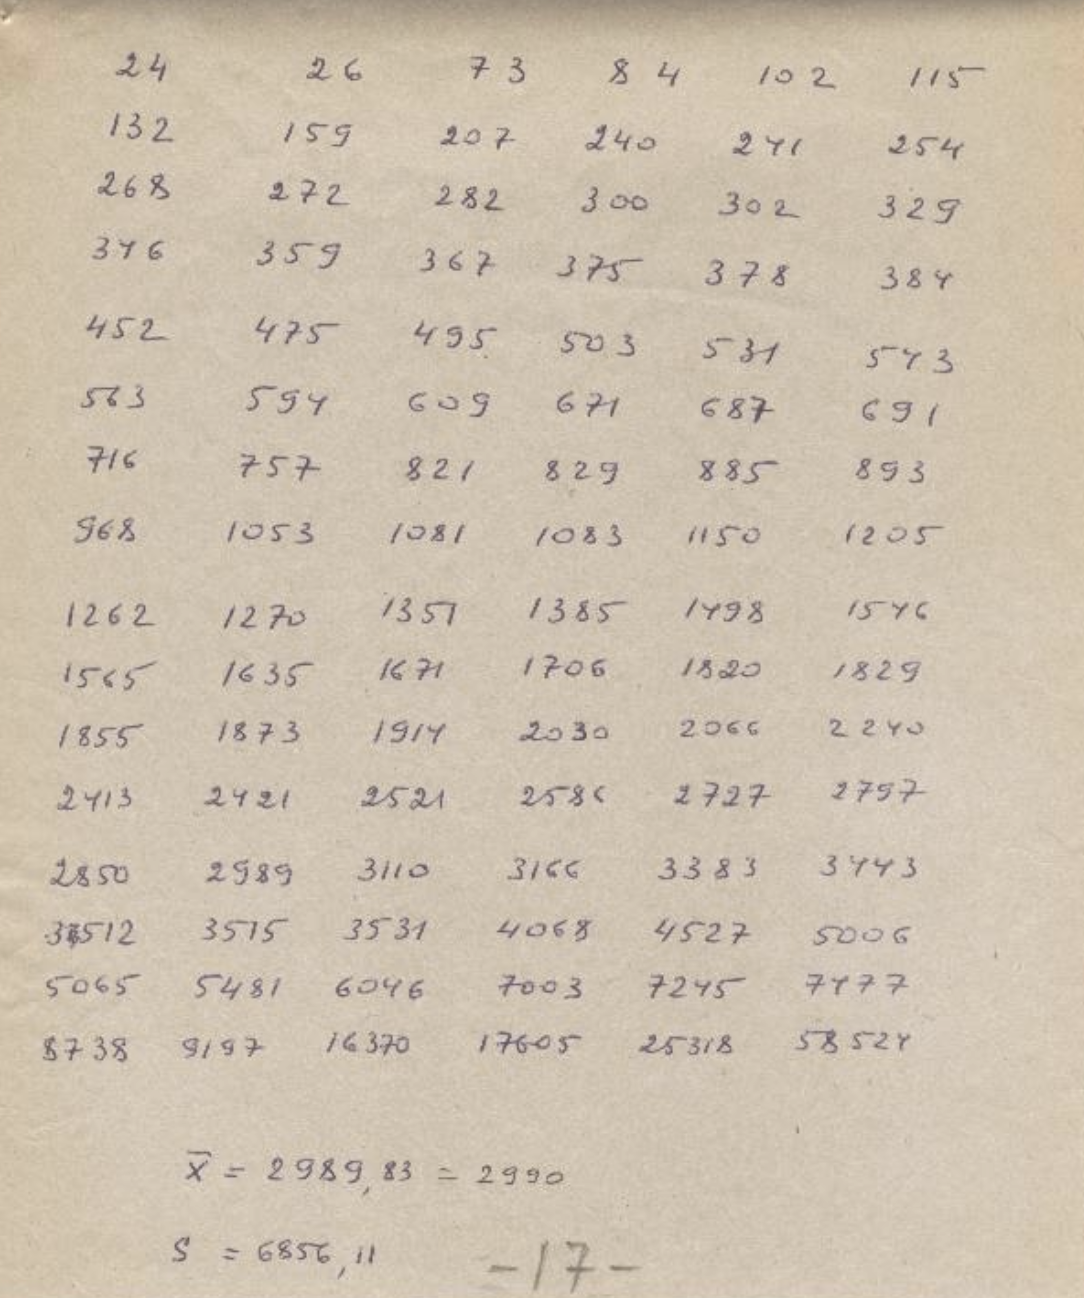
\includegraphics[scale=0.8]{pic1}
\caption{Таблица страховых возмещений}
\end{figure}



\begin{center}
	\begin{tabular}{ |c|c|c|c|c|c|} 
	 \hline
	 Стоим. возм. & набл.част. & теор.част.(эксп.) &  Pareto a) & Pareto b) & Weibull $W(c,\gamma)$ \\
	 \hline 
	 0-260 & 12 & 8 & 12.7 & 15.4 & 17.6 \\ 
	 \hline
	260 - 545 & 18 & 8 & 11.4 & 13.0 & 11.9 \\ 
	 \hline
	 545 - 860 & 10 & 8 & 10.2 & 10.9 & 10.0\\ 
	 \hline
	 860 - 1212 & 8 & 8 & 9.1 & 9.3 & 8.8 \\ 
	 \hline
	 1212 - 1612 & 7 & 8 & 8.2 & 8.0 & 7.9 \\ 
	 \hline
	 1612 - 2073 & 10 & 8 & 7.4 & 6.9 & 7.1 \\ 
	 \hline
	 2073 - 2618 & 5 & 8 & 6.7 & 6.0 & 6.5 \\ 
	 \hline
	 2618 - 3285 & 6 & 8 & 6.1 & 5.3 & 6.0 \\ 
	 \hline
	 3285 - 4145 & 6 & 8 & 5.6 & 4.8 & 5.5 \\ 
	 \hline
	 4145 - 5357 & 3 & 8 & 5.2 & 4.4 & 5.1 \\ 
	 \hline
	 5357 - 7430 & 4 & 8 & 5.1 & 4.2 & 4.8 \\ 
	 \hline
	 7430 - $\infty$ & 7 & 8 & 8.3 & 7.7 & 4.8 \\ 
	 \hline
	\end{tabular}
\end{center}


Строим гистограмму:

\begin{figure}[h!]
\centering
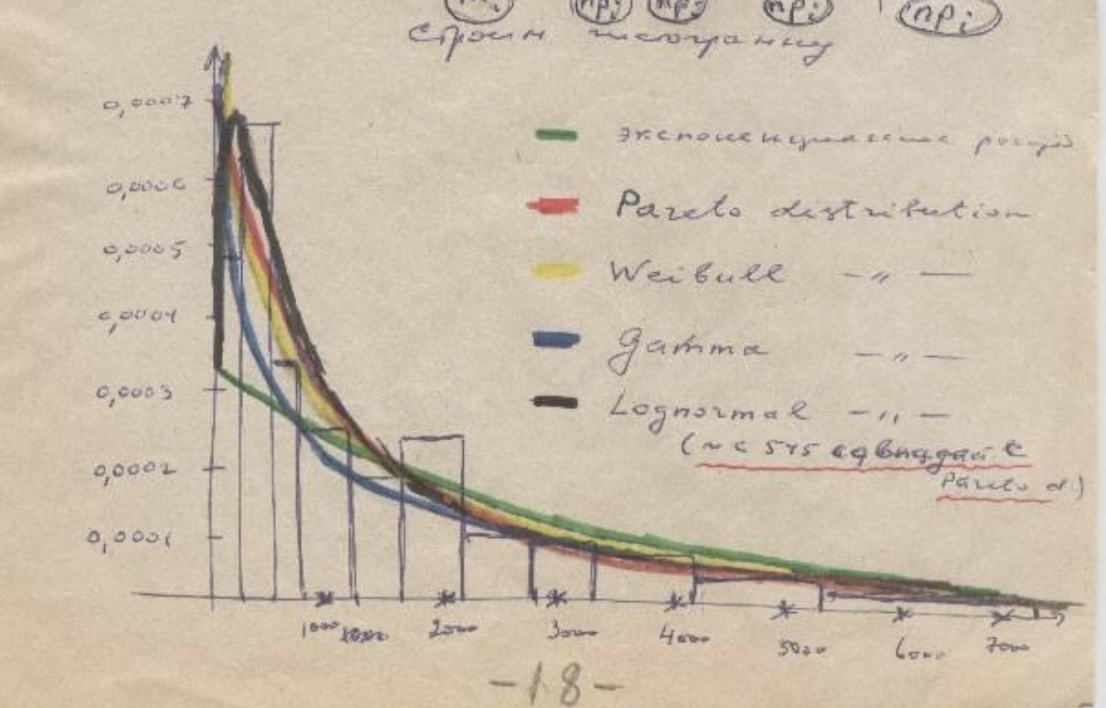
\includegraphics[scale=0.8]{pic2}
\caption{Гистограмма}
\end{figure}


Первоначальный общий вывод о типе распределения : оно ассиметричное с длинным хвостом.

\subsection{Экспоненциальное распределение} % (fold)
Пусть $\overline{\lambda} $ оценка параметра $\lambda$. Используя метод максимального правдоподобия , найдем, что
\[ \overline{\lambda} = \overline{X} = \frac{\sum X_i}{n}.\]

Для нашего случая $\overline{X} = 2990 = \overline{\lambda}. $

Проверяем гипотезу об экспоненциальном распределении с параметром $\overline{\lambda} = 2990  
.$

Проверяем с помощью критерия $\chi^2 = \sum\limits_{i=1}^{12}\frac{(m_i - np_i)^2}{np_i}$.

Весь интервал разбит на 12 интервалов, $m_i$ известны,$np_i$ подсчитываем. Получаем $\chi^2 = 23$ (у нас $\chi^2$ с 12 - 1 -1 = 10 степенями свободы). Тогда
\begin{gather*}
	\alpha = 0.01 \;\; \chi^2_{1-\alpha} = 23.2 \;\Rightarrow\;\; \text{ гипотеза отбрасывается}\\
	\alpha = 0.05 \;\; \chi^2_{1-\alpha} = 18.31
\end{gather*}

% subsection экспоненциальное_распределение (end)

% section распределения_потерь (end)
% section нетто_ставка_страхового_взноса (end)


% section апостериорное_распределение_числа_требований_на_t_t_ (end)
% section система_бонус_малус (end)
% subsection распределение_пуассона (end)
% section распределения_для_числа_страховых_требований (end)
% chapter лекция_6_страхование_не_жизни (end)